\documentclass[10pt,mathserif]{beamer}
\usepackage[english]{babel}
\usepackage[utf8]{inputenc}
\usepackage[T1]{fontenc}
\usepackage{cmbright}
\usepackage{tikz}
\usepackage{listings}
\usepackage{relsize}

\usetikzlibrary{arrows}
\usetikzlibrary{backgrounds}
\usetikzlibrary{chains}
\usetikzlibrary{fit}
\usetikzlibrary{positioning}
\usetikzlibrary{scopes}
\usetikzlibrary{trees}

\usetheme{Warsaw}
\useoutertheme{essential}
\setbeamertemplate{navigation symbols}{}

\author{Stefano Cherubin}
\institute{Politecnico di Milano}
\date{08-05-2019}
\title{Quick start: LLVM compiler framework}
\newcommand{\customdata}{Stefano Cherubin <stefano.cherubin@polimi.it>}
\renewcommand{\ttdefault}{pxtt}
\lstset{basicstyle=\ttfamily\scriptsize}
\newcommand{\cinput}[1]{\lstinputlisting[language=C]{#1}}
\newcommand{\cinline}[1]{\lstinline[language=C]!#1!}
\newcommand{\llvminput}[1]{\lstinputlisting[language=LLVM]{#1}}
\newcommand{\llvminline}[1]{\lstinline[language=LLVM]!#1!}
\lstdefinelanguage{LLVM}%
  {morekeywords={define,declare,global,constant,internal,external,private,%
      linkonce,linkonce_odr,weak,weak_odr,appending,common,extern_weak,%
      thread_local,dllimport,dllexport,hidden,protected,default,except,deplibs,%
      volatile,fastcc,coldcc,cc,ccc,x86_stdcallcc,x86_fastcallcc,ptx_kernel,%
      ptx_device,signext,zeroext,inreg,sret,nounwind,noreturn,nocapture,byval,%
      nest,readnone,readonly,noalias,uwtable,inlinehint,noinline,alwaysinline,%
      optsize,ssp,sspreq,noredzone,noimplicitfloat,naked,alignstack,module,asm,%
      align,tail,to,addrspace,section,alias,sideeffect,c,gc,target,datalayout,%
      triple,blockaddress},%
  morekeywords=[2]{add,fadd,sub,fsub,mul,fmul,sdiv,udiv,fdiv,srem,urem,frem,%
     and,or,xor,icmp,fcmp,eq,ne,ugt,uge,ult,ule,sgt,sge,slt,sle,oeq,ogt,oge,%
     olt,ole,one,ord,ueq,ugt,uge,ult,ule,une,uno,nuw,nsw,exact,inbounds,phi,%
     call,select,shl,lshr,ashr,va_arg,trunc,zext,sext,fptrunc,fpext,fptoui,%
     fptosi,uitofp,sitofp,ptrtoint,inttoptr,bitcast,ret,br,indirectbr,switch,%
     invoke,unwind,unreachable,malloc,alloca,free,load,store,getelementptr,%
     extractelement,insertelement,shufflevector,extractvalue,insertvalue},%
  sensitive=t,%
  morestring=[b]",%
  morecomment=[l];%
  }[keywords,comments,strings]

\AtBeginSection[]
{
\begin{frame}{Contents}
\tableofcontents[currentsection]
\end{frame}
}
\begin{document}

\begin{frame}
\maketitle
%\begin{center}
%\itshape\scriptsize This material is strongly based on Ettore Speziale's material \textsl{}for the previous year course.
%\end{center}
\end{frame}

\section{Introduction}
\begin{frame}{Understanding LLVM}
	\begin{center}
	\huge{
		LLVM is not a compiler.\\
		\pause
		\vfill
		LLVM is a collection of components\\
		which is useful to build a compiler.
	}
	\end{center}
\end{frame}

\begin{frame}{Getting LLVM}
\begin{itemize}
	\item ``old'' git mirrors
		\begin{itemize}
			\item only llvm repo (subprojects in separated repos, can be added later)
			\item \texttt{git clone -b release\_80 --single-branch git@github.com:llvm-mirror/llvm.git}
		\end{itemize}
	\vfill
	\item ``new'' git monorepo
		\begin{itemize}
			\item all in one repo (llvm + major subprojects)
			\item \texttt{git clone -b release/8.x --single-branch git@github.com:llvm/llvm-project.git}
		\end{itemize}
\end{itemize}
\end{frame}

\begin{frame}{What LLVM is made of}
\begin{itemize}
	\item C++ libraries
		\begin{itemize}
			\item \texttt{src/include/llvm/...}
			\item \texttt{src/lib/...}
		\end{itemize}
		\vfill
	\item small application (tools)
		\begin{itemize}
			\item \texttt{src/tools/...}
			\item \texttt{src/utils/...}
		\end{itemize}
\end{itemize}
\vfill
You can find binaries of them in the installation directory under \texttt{root/bin/...}
\end{frame}

\begin{frame}{clang}
\begin{itemize}
	\item \texttt{clang} is a compiler based on LLVM
	\item It compiles all major C-like languages
	\vfill
	\item It is part of the git monorepo
	\item It can be added as a tool in the LLVM framework but must be manually cloned in the tool directory
	\begin{enumerate}
		\item \texttt{cd src/tools}
		\item \texttt{git clone http://llvm.org/git/clang} (git mirror version)
	\end{enumerate}
	\vfill
	\item You can easily see on a production quality compiler the impact of changes you made on your local copy of LLVM
\end{itemize}
\end{frame}

\section{LLVM framework quick start}
\begin{frame}{Commands}
	\begin{description}
		\item[llvm-as] LLVM assembler
		\item[llvm-dis] LLVM disassembler
		\item[opt] LLVM optimizer
		\item[llc] LLVM static compiler
		\item[lli] directly execute programs from LLVM bitcode
		\item[llvm-link] LLVM bitcode linker
		\item[llvm-mca] LLVM machine code analyzer
		\item[llvm-nm] list LLVM bitcode and object file's symbol table
		\item[llvm-stress] generate random .ll files
		\item[llvm-config] prints out install configuration parameters
		\item[llvm-dwarfdump] print contents of DWARF sections
	\end{description}
	\vfill
	For a complete reference, see LLVM command guide \footnote{\url{http://llvm.org/docs/CommandGuide/index.html}}
\end{frame}

\begin{frame}
	\noindent\hspace{-1.2cm}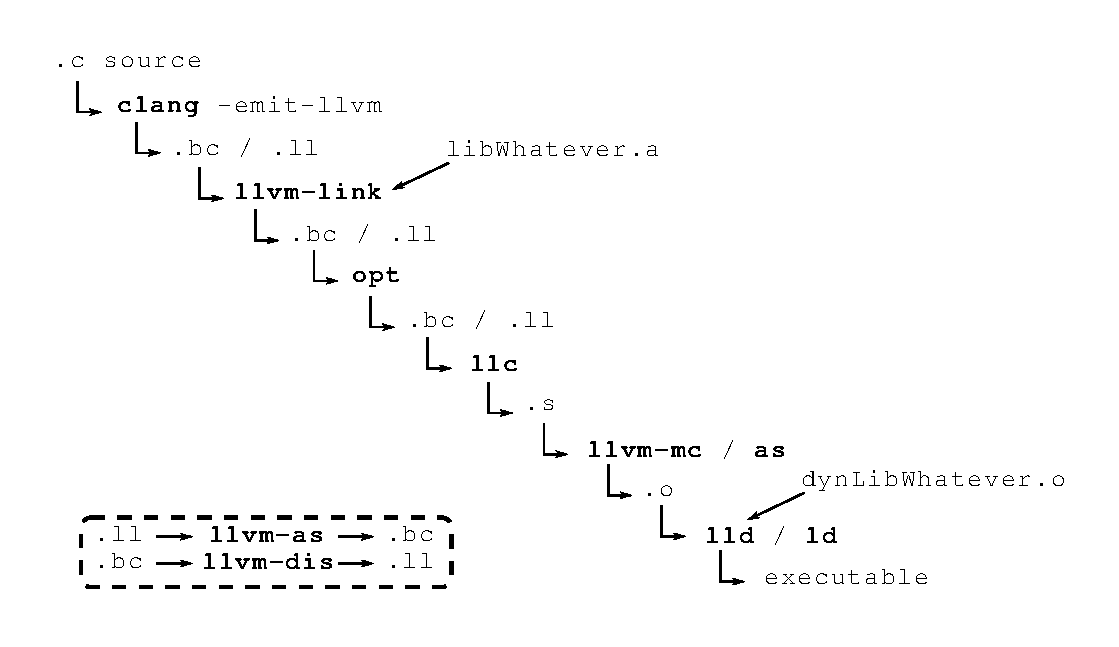
\includegraphics[width=13cm]{img/03/toolchain}
\end{frame}

\begin{frame}{Writing a LLVM pass}
	There are a lot of tutorials available:
	\vfill
	\begin{itemize}
		\item Official developer guide\\ \href{http://llvm.org/docs/WritingAnLLVMPass.html}{\url{llvm.org/docs/WritingAnLLVMPass}}
		\vfill
		\item Out-of-source pass\\ \href{https://github.com/quarkslab/llvm-dev-meeting-tutorial-2015}{\url{github.com/quarkslab/llvm-dev-meeting-tutorial-2015}}
	\end{itemize}
	\vfill
	We will follow the first one, with a few adjustments.
\end{frame}

\begin{frame}{Testing}
LLVM has an internal testing infrastructure. \footnote{\url{http://llvm.org/docs/TestingGuide.html}}
Please use it.
\\
\begin{description}
	\item[llvm-lit] LLVM Integrated Tester
\end{description}
\begin{enumerate}
	\item Forge a proper LLVM-IR input file (.ll) for your test case
	\item Instrument it with \texttt{lit} script comments
	\item Run \texttt{lit} on your test
		\begin{itemize}
			\item \texttt{llvm-lit ~/llvm/test/myTests/singleTest.ll}\\ run a single test
			\item \texttt{llvm-lit ~/llvm/test/myTests}\\ run the test suite (folder)
		\end{itemize}
	\item Run \texttt{lit} on the LLVM test suite (regression testing)
\end{enumerate}
\vfill
To submit a bug report to LLVM developers you will be asked to write a \texttt{lit} test case that highlights the bug.
\end{frame}

\end{document}
